\section{Search Problems}

\subsection{Definition}
\begin{frame}{What is Search?}
  In daily life, we {\bf search} for something when we are trying to find where this thing is located.\medskip

  \begin{itemize}
  \item Keys of your bycicle;
  \item Your wallet;
  \item Your cellphone;
  \end{itemize}\medskip

  The search has an {\bf Objective} (what are we searching?), and the {\bf search space} (where can we search?).

  \begin{block}{}
    {\smaller
    \hfill \emph{The thing you search is always in the last place you look}\\
    \hfill (\emph{By definition!})}
  \end{block}
\end{frame}

\begin{frame}
  \frametitle{What is a ``Search Problem''?}
    A {\bf search problem} is a problem that we can describe as: "check many {\bf possible answers} until you find a {\bf solution}".\bigskip

    \begin{itemize}
      \item One answer to a search problem can be {\bf correct} or {\bf incorrect};\smallskip

      \item In some search problems, an answer can have a {\bf quality score};\smallskip

      \item The {\bf set of answers} to a search problem can be {\bf sorted} by some criteria;
    \end{itemize}
    \bigskip

    Many problems in programming challenges (and also in real life) can be described as search problems. We can apply very simple {\bf search algorithms} to solve these problems.
\end{frame}

\begin{frame}{Search Problem Examples (from past weeks)}
  We can {\bf calculate} the answer, which is usually very fast,\\
   or we can {\bf search} the answer, which is usually slow.

  \begin{block}{Traffic Lights (Week 1)}
    {\bf Objective:} FIND the time (in seconds) when all the different lights are synchronized at green.
    \bigskip

    {\bf Search Space}: Time $s$ from 1 to 18000.
  \end{block}

  \begin{block}{File Fragmentation (Week 2)}
    {\bf Objective:} Given a set of binary fragments, FIND the binary string that matches every pair.
    \bigskip

    {\bf Search Space:} All binary strings from $x = 0$ to $x = 2^{n-1}$.
  \end{block}
\end{frame}


\begin{frame}
  \frametitle{The Generic Search Algorithm}
  Any problem that can be described as a {\bf Search Problem} can also be solved using a {\bf Search Algorithm}.
  \begin{enumerate}
    \item Sort and order the search space; $n = 1$
    \item Generate the $n^{\text{th}}$ answer: $a_n$.
    \item Test if $a_n$ is a solution to the problem;
    \item $n = n+1$, go back to 2.
  \end{enumerate}\bigskip

  Some questions when you program the search algorithm:
  \begin{itemize}
  \item How to generate one answer? How many answers we store in memory?
  \item How many answers exist in total? How to order the search space?
  \item Is it possible to skip some answers? (pruning)
  \item How many solutions are necessary?
  \end{itemize}
\end{frame}

\subsection{Example}
\begin{frame}[fragile]{Search Problem Example}{File Fragmentation}
  Let's use this algorithm to last week's "File Fragmentation".\medskip

  We find the correct size of the answer, and we test each binary string
  of that size.\\
  To do that, we check if it fits all the fragments.

  \begin{columns}[T]
    \column{0.5\textwidth}
  \begin{block}{Input -- A Set of binary fragments}
\begin{verbatim}
0011
100
1100
00
00
001
\end{verbatim}
  \end{block}
     \column{0.5\textwidth}
  \begin{exampleblock}{Output -- one bin string that fit all}
\begin{verbatim}
000000  ->  0011 + 00   X
000001  ->  0011 + 00   X
  ...
001100  ->  0011 + 00   OK
            00 + 1100   OK
            001 + 100   OK!
\end{verbatim}
  \end{exampleblock}
\end{columns}\bigskip

  How long does would this algorithm take?
\end{frame}

\begin{frame}{Search Problem Example}{File Fragmentation -- Considerations}
  Using this {\bf Full Search} algorithm, we can find a solution to the File Fragmentation problem. However, how long does this algorithm take?\medskip

  \begin{itemize}
  \item \structure{What is the search space?}\\
    The search space is every binary string $B$ of max size $n$. $(O(2^n))$
    \bigskip

  \item \structure{How to check one answer?}\\
    We test all combinations of 2 out of $m$ fragments. $O(C_{m,2})$
    \bigskip

  \item \structure{What is the expected running time?}\\
    We need to check every solution: $2^n \times C_{m,2} =  O(2^nC_{m,2})$
  \end{itemize}
  \bigskip

  We calculate the running time of the algorithm using $n$ and $m$
\end{frame}

\begin{frame}{Search Problem Example}{Let's practice some simple search problems!}

  \begin{block}{Consider the same input for all problems}
    You have unsorted an array $A$ with $n$ integers ($n < 10.000$).\\
    Each $a_i$ is in \{$0 \leq a_i \leq 100.000$\}.
  \end{block}\bigskip

  For each problem below, what is the expected running time of a full search?
  \begin{enumerate}
  \item Find the {\bf largest} and the {\bf smallest} element of $A$;
  \item Find the {\bf $k^{th}$ smallest} element of $A$;
  \item Find the {\bf largest gap} $G$; where $x,y \in A$ and $G = |x-y|$;
  \item Find the {\bf longest increasing subsequence (LIS)} of A;\\
    \hfill Example of LIS: $A = [3,2,5,\overline1,4,\overline{2, 3, 5},7,\overline{6,10}]$
  \end{enumerate}
\end{frame}

\begin{frame}{Search Problem Example}{Let's practice!}
  What is the expected running time of each problem?
  \begin{enumerate}
  \item {\bf Find the Largest and smallest element of $A$:}
    \begin{itemize}
      \item $O(n)$: a full pass over all numbers.
    \end{itemize}
  \item {\bf Find the $k^{th}$ smallest elements of $A$:}
    \begin{itemize}
      \item Repeat the full pass $k$ times, remove smallest each time. $O(nk)$, or $O(n^2)$ in worst case;
      \item Sort A and list first $k$ elements: $O(n\log{n})$
    \end{itemize}
  \item {\bf Fing the largest gap:}
    \begin{itemize}
    \item Try all possible pairs: Two loops: $O(n^2)$
    \item Find the smallest and largest numbers $O(n)$ (proof: largest gap = biggest - smallest)
    \end{itemize}
  \item {\bf Longest increasing subsequence:}
    \begin{itemize}
    \item Test all possible subsequences: $O(2^n)$
    \item Dynamic programming: $O(n^2)$
    \item Greedy search: $O(n\text{log}k)$ -- Look for this algorithm!
    \end{itemize}
  \end{enumerate}
\end{frame}
% TODO: Add the slide for LIS with greedy here for reference, or maybe
% in the greedy section

\section{Search Algorithms}

\begin{frame}{}{}
  \begin{center}
    {\bf Part II: Search Algorithms}
  \end{center}
\end{frame}

\begin{frame}
  \frametitle{Search Algorithm Paradigms}
  There are many variations on Search Algorithm:
  \bigskip

  \begin{itemize}
    \item Complete Search/Brute Force;
    \item Divide and Conquer;
    \item Greedy Approach;
    \item Dynamic Programming (Next week!)
    \item Heuristic Search (not in this course!)
    \item Meta-heuristic Search (not in undergraduate school!)
    \item ... and many others.
  \end{itemize}
  \bigskip

  Depending on the problem, we can use different approaches. Which approach is better depends on the problem, so let's learn some of them.
\end{frame}


\subsection{Complete Search}

\begin{frame}{Complete Search}{Definition}

  The search algorithm we used until now is the {\bf Complete Search}.\\
  A Complete Search algorithm checks all the solutions in the search space of the problem.\bigskip

  Another name for Complete Search algorithms is {\bf Brute Force}. Brute force sounds negative, but Complete Search algorithms have some uses, so we will use a "nicer" name.
\end{frame}


\begin{frame}{Complete Search}{Structure}

  The structure of a Complete Search algorithm is very simple:
  \bigskip

  \begin{itemize}
    \item {\bf Define or List all possible answers}\\
    Choose the right data structure that contains all answers.
    \bigskip

  \item {\bf Check each answer if it is a solution}\\
    Normally using a loop or recursive function;
    \bigskip

  \item {\bf Prune, Prune, Prune}\\
    They key to a fast Complete Search algorithms is to reduce the number of answers.\\

    In the program, we can do this using "break" in loops, or using early "return" clauses in recursive functions.
  \end{itemize}

\end{frame}

\begin{frame}{Complete Search}{Example: UVA 725 -- Division}
  \begin{block}{Problem Summary}
    You receive an integer $N$. You have to find all pairs of numbers with 5 digits ($abcde$ and $fghij$) that satisfy two conditions:
    \begin{enumerate}
      \item $fghij / abcde = N$
      \item $a,b,c,d,e,f,g,h,i,j$ are all different.
    \end{enumerate}
  \end{block}\bigskip

  {\bf Example:} $N = 62$
  \medskip

  79546 / 01283 = 62\\
  94736 / 01528 = 62\\
  \bigskip

  \begin{alertblock}{QUIZ!}
    Think: How can you solve this problem using {\bf Complete Search}?
  \end{alertblock}
\end{frame}

\begin{frame}[fragile]{Complete Search Example: UVA 725 Division}{Naive Solution}
  \begin{block}{}
    Test all $x$ where $0 \leq x \leq 99999$, calculate $y = x*n$, and test if all digits of $x$ and $y$ are different.
  \end{block}

{\smaller
\begin{verbatim}
for (int x = 0; x <= 99999; x++) {
  y = x*n;
  digits = count_digits(x,y);
  if (digits == 1<<10 - 1) printf("%0.5d/%0.5d=%d\n",y,x,N);
}

int count_digits(int x, int y) {
  int used = (x < 10000); % bit array: each bit mark one digit
  int tmp;
  tmp = x; while (tmp) {used |= 1 << (tmp%10); tmp /= 10; }
  tmp = y; while (tmp) {used |= 1 << (tmp%10); tmp /= 10; }
  return used;
}
\end{verbatim}
  }
\end{frame}

\begin{frame}{Complete Search Example: UVA 725 Division}{Prunning the Loop}
  The algorithm in the previous slide is {\bf very slow}.\\
  The loop tests many numbers that will {\bf never} be the right answer.\bigskip

  How can we prune (reduce) the number of answers that we test?\bigskip

  \begin{itemize}
  \item What is the absolute minimum and maximum values of $x$?\\
    \hspace{1cm} 01234 to 98765 \hspace{2cm} (different digits)
    \bigskip

  \item Maximum for $y$ is also 98765, so the real maximum for $x$ is less:\\
    \hspace{1cm} $x_{\text{max}} = 98765/N$, \hspace{1.8cm} $($remember: $x * y = N)$
    \bigskip

  \item Can you think of other ways to prune?
  \end{itemize}
\end{frame}

\begin{frame}
  \frametitle{Notes about Complete Search algorithms}
  \begin{itemize}
  \item A Complete Search should always give the correct solution (if bug free)\\
    \begin{itemize}
    \item It checks all answers, so it should always find the correct one;
    \item Checking all answers usually takes too long;
    \end{itemize}

    \bigskip

  \item For some problems, the Complete Search is the right algorithm.
    \begin{itemize}
    \item The problem is so small, so a Complete Search is the simplest solution.
    \item Prune, prune, prune!
    \end{itemize}

    \bigskip

  \item For a very hard problem, a Complete Search can give you a starting point;
    \begin{itemize}
    \item Maybe the Complete Search will be "time limited exceeded";
    \item But you can use Complete Search to generate "test cases";
    \end{itemize}
  \end{itemize}
\end{frame}

\begin{frame}
  \frametitle{Complete Search Example 2: Simple Equations}
  \begin{block}{Problem Summary -- UVA 11565}
    {\bf Input:} A, B, C, $1 \leq A,B,C \leq 10000$.\bigskip

    Find $x,y,z$ so that:
    \begin{itemize}
    \item $x+y+z=A$,
    \item $x*y*z=B$,
    \item $x^2+y^2+z^2=C$,
    \end{itemize}

    \bigskip
  \end{block}
  \bigskip

  To solve this problem we can loop and test on of x, y, z (3-nested loop).
  \bigskip

  But what should be the minimum and maximum value of the loops?
\end{frame}

% First take x^2+y^2+z^2 = C. Since maximum C is 10000, and X,Y,Z must be
% different, the maximum range of x is -100 to 100. The Reasoning goes for
% Y and Z. With this we can do a triple loop with about 8M operations.

\begin{frame}[fragile]{Complete Search Example 2: Simple Equations}{Initial Pruning}
  \begin{block}{}
    Consider $x^2 + y^2 + z^2 = C$.\medskip

    Since $C \leq 10000$, and $x^2,y^2,z^2 \geq 0$, if $y =
    z = 0$ then the range for $x$ must be $-100, 100$.
  \end{block}

{\smaller
\begin{verbatim}
int x,y,z;
for (x = -100; x <= 100 && !sol; x++)
  for (y = -100; y <= 100 && !sol; y++)
    for (z = -100; z <= 100 && !sol; z++)
      if (y != x && z != x && z != y &&
          x + y + z == A && x * y * z == B &&
          x*x + y*y + z*z == C) {
             printf("%d %d %d\n", x,y,z);
             exit(0);
          }
\end{verbatim}}

\begin{block}{}
  QUIZ: How can we prune this loop even more?
\end{block}
\end{frame}

\begin{frame}{Complete Search Example 2: Simple Equations}{More Pruning}
  There are many other ways that we can prune the loop:

  \medskip

  \begin{itemize}
  \item We can change the range using the actual input values of $A,B,C$
  \item We only need one solution. We can break the loop once we find it.
  \item We can use equation 2 to think of other ways to prune.
  \end{itemize}

  \vfill

  % \begin{alertblock}{}
  %   The problem: ``Simple Equations -- Extreme!'' has a much
  %   higher range for $A,B,C$. You need a lot of pruning to avoid a TLE!
  % \end{alertblock}
\end{frame}

\begin{frame}
  \frametitle{Complete Search Tips}
  Main question about Complete Search: Is the program fast enough?
  \bigskip

  To make your program faster, find the {\bf critical part} of the code, and improve that first!
  \vfill

  \begin{block}{Tip 1 -- Filtering Vs Generating}
    {\bf Filter Programs} examine all answers and remove
    incorrect ones. Generally iteractive. Generally easier to
    code. Example: Request for proposal.

    \bigskip

    {\bf Generating Programs} gradually build answers and
    prune invalid partial answers. Generally recursive. Generally
    faster. Example: 8 queens.
  \end{block}
\end{frame}

\begin{frame}
  \frametitle{Complete Search Tips}
    \begin{block}{Tip 2 -- Prune Early}
      In the N queen problem, if we imagine a recursive solution that
      places 1 queen per column, we can prune rows, columns and
      \structure{DIAGONALS}.

      \smallskip

      Also remember to mark impossible places when you enter the
      recursion, and unmark when you leave, using bitmasks.
      %%% 2.A - Finding simmetries can help, but it is often not worth the troube.
    \end{block}

    \vfill

    \begin{block}{Tip 3 -- Pre-computation}
      Sometimes it is possible to generate tables of partial solutions.

      \medskip

      Load this data in your code to accelerate computation (at the
      expense of memory). The programming cost is high, since you have
      to output the tables in a way to facilitate putting it in the
      code.
    \end{block}
\end{frame}


\begin{frame}%% TODO: Expand on this example
  \frametitle{Complete Search Tips}
    \begin{block}{Tip 4 -- Solve the problem backwards}
      Sometimes a less obvious angle of attack may be easier.
      \bigskip

      {\bf Example:} "Rat Attack". A city with 1024 x 1024 blocks has $n \leq 20000$ rats in some of its blocks. You have a bomb with radius $d \leq 50$. Where do you place the bomb to kill most rats?
      \bigskip

      {\bf Obvious Approach}: Check the radius of the bomb ($50^2$) at each of the $1024^2$ blocks.\\ Cost: $1024^2 \times 50^2 = 2.62\times 10^9$
      \bigskip

      {\bf Backwards Approach}: Make a 1024x1024 matrix of ``killed rats''. For each rat, add it to each cell in the bomb radius.\\
      Cost: Number of rats ($n$) and bomb radius ($d$)\\
      $n * d^2 = 20000*2500 = 5\times10^7 + 1.048\times10^6$.
    \end{block}
\end{frame}

% \begin{frame}
%   \frametitle{Complete Search Tips}
%     \begin{block}{Tip 5 -- Optimizing the source code}
%       \begin{itemize}
%       \item Loops are usually faster than recursion
%       \item Using built-in data types is usually faster than arrays/vectors
%       \item Printf is usually faster than CIN/COUT
%       \item Many other tips
%
%         \bigskip
%
%       \item Don't forget the Time Optimization vs. Programmer
%         Optimization tradoff!
%       \end{itemize}
%
%     \end{block}
% \end{frame}

%%%% 3.3 Divide and conquer

\section{Divide and Conquer}

\begin{frame}
  \begin{center}
    {\bf Part III -- Divide and Conquer, and Greedy Algorithms}
  \end{center}
\end{frame}

\begin{frame}
  \frametitle{Divide and Conquer}



  Divide and Conquer (D\&C) is a problem-solving paradigm in which a
  problem is made simpler by 'dividing' it into smaller parts.\bigskip

  \begin{itemize}
  \item Divide the original problem into sub-problems;
  \item Find (sub)-solutions for each sub-problems;
  \item Combine sub-solutions to get a complete solution;
  \end{itemize}\bigskip

  \begin{block}{Examples}
    Quick Sort, Binary Search, etc...
  \end{block}
\end{frame}

\begin{frame}
  \frametitle{Canonical Divide and Conquer}
  \begin{enumerate}
  \item Sort an static array;
  \item You want to find item $n$.
  \item Test the middle of the array.
  \item If $n$ is smaller/bigger than the middle, throw away the second/first half.
  \item Repeat
  \end{enumerate}

  \vfill

  Search time: O(log n) plus sorting time if necessary.
\end{frame}

%\begin{frame}
%  \frametitle{Binary Search on Uncommon Data St
%\end{frame}

%%% Binary Search on Uncommon Data Structures
%% Example: Parents in a tree: Find the parent of node V that has value over P
% which is closest to the root. Q <= 20K, N <= 80K
%% Naive approach: For each note, search all parents. Worst case is QN (TLE)
%% Divide and conquer approach: Take each path from the root, and solve all
% Queries for each root, using binary search == O(QlogN)

\begin{frame}
  \frametitle{Binary Search on Simulation Problems}

  Simulation problems usually require us to find a value that solves
  a complex simulation.

  \begin{block}{Problem Example: Paying the debt}
    You have to pay $V$ dollars. You pay $D$ dollars per month, in $M$
    months. Each month, before paying, your debt increases by $i$.

    \medskip

    If we fix $M$,$I$ and $V$, what is the minimal $D$?
  \end{block}

  \bigskip

  $V = 1000$, $M = 2$, $i = 1.1$, what is the minimum $D$?

  \begin{itemize}
  \item $D = 500$:
    \begin{itemize}
    \item $m_1: V_0 *1.1 - D = 600, m_2: v_1*1.1 - D = 160$
    \end{itemize}
  \item $D = 600$:
    \begin{itemize}
    \item $m_1: V_0 *1.1 - D = 500, m_2: v_1*1.1 - D = -50$
    \end{itemize}
  \end{itemize}
\end{frame}

\begin{frame}
  \frametitle{How to approach the Simulation Problem?}

  {\bf Possible Approaches:}
  \begin{itemize}
  \item Complete Search (what about continuous search space?)
  \item Find the derivative of the simulation and solve it to zero;
  \item Start from the end state of the simulation and calculate back;
  \item \alert{These approaches can be hard for complex simulations!}
  \end{itemize}

  \bigskip

  {\bf Binary Search Approach:}
  \begin{enumerate}
  \item Estimate a minimum and maximum possible answer $(a,b)$
  \item Choose the middle value as an answer and simulate it;
  \item Adjust the limits $(a,b)$ based on simulation result;
  \item Go back to 2.
\end{enumerate}
\end{frame}

\begin{frame}
  \frametitle{Binary Search for Simulation}
{\bf Input:} $m = 2, v = 1000, i = 0.1$\bigskip

\begin{itemize}
  \item Choose initial range: (ex: [0.01 to 1100.00]); Initial $d$: 550.005
  \item $f(d,m,v,i) = \text{loop}(v*(1+i) - d)$, $m$ times
  \item Do binary search in this range;
\end{itemize}
\bigskip

{\smaller
\begin{tabular}{c|c|c|c|l}
 a & b & d & simulation: f(d,m,v,i) & action: \\
 \hline
 0.01 & 1100.00 & 550.005 & error: -54.98 & increase a\\
 550.005 & 1100.00 & 825.002 & error: 522.50 & decrease b\\
 550.005 & 825.002 & 687.503 & error: 233.75 & decrease b\\
 550.005 & 687.503 & 681.754 & error: 89.38 & decrease b\\
 550.005 & 618.754 & 584.379 & error: 17.19 & decrease b\\
 550.005 & 584.379 & 567.192 & error: -18.89 & increase a\\
 567.192 & 584.379 & 575.786 & error: -0.84 & increase a\\
 ... & ... & ... & a few iterations later ... & ...\\
 ... & ... & 576.190 & error $< \epsilon$ & stop: answer = 576.19\\
\end{tabular}}
\bigskip

Total number of steps: $O(log_2((b-a)/\epsilon))$
\end{frame}

% \begin{frame}
%   \frametitle{Bisection Method Principle}
%
%   \begin{itemize}
%   \item {\bf Principle}: Search on the solution space and test the answer.
%     \bigskip
%
%   \item Another example: UVA 11936 - Through the desert
%     \bigskip
%
%   \item This technique requires the solution space to be \alert{Unimodal}
%   \end{itemize}
% \end{frame}

%%%% 3.4 Greedy
\subsection{Greedy}
\begin{frame}
  \frametitle{The Greedy Search Algorithm}

  \begin{block}{Definition}
    A {\bf Greedy Search Algorithm} will make the \alert{locally optimal choice} at each step of the program, with the hope that eventually it will reach the \alert{globally optimal solution}.
  \end{block}
  \vfill

  Greedy can be very fast, or very wrong. For a greedy algorithm to work, a problem must show two properties:
  \begin{itemize}
  \item It has optimal sub-structures. In other words: an answer to the search problem must have {\bf local steps that can be evaluated};

  \item It has the {\bf greedy property}: If you always choose the local step with the highest evaluation, you will "eventually" reach the optimal solution.
  \end{itemize}
  \bigskip

  The first property is similar (but not identical) to dynamic programming. The second property is harder to prove.
\end{frame}

\begin{frame}
  \frametitle{Greedy Search Example: Minimal Coverage}

  \begin{block}{}
    Consider an interval [A,B], and a set of $n$ intervals $S =
    [(a_1,b_1), (a_2,b_2), \ldots (a_n,b_n)]$.

    \medskip

    Find the minimal subset
    of $S$ which completely covers [A,B].
  \end{block}

  \bigskip

  \begin{itemize}
  \item A = 10, B = 50;\bigskip


  \item S = [(5,15), (8,12), (40,60), (30,40), (20,40), (13,25),
    (33,55), (18,30)]
  \end{itemize}

  \[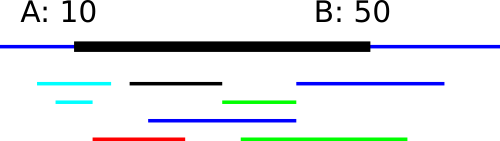
\includegraphics[width=0.6\textwidth]{img/minimal_coverage}\]
\end{frame}

\begin{frame}{Greedy Search Example: Minimal Coverage}{Search Algorithm}
  The algorithm that solves this problem progressively adds items to cover the area from left to right. It starts with a solution set $C = \emptyset$, and cover point $A_c = A$.
  \bigskip

  \begin{enumerate}
    \item Find and remove subset $S_c \subset S$, of all intervals that cover $A_c$;\\
      {\smaller \hfill(if $S$ is sorted by left value, this is fast)}
    \item Choose the interval $s_i \in S_c$ with the {\bf maximum} left value.
    \item Update $A_c$ with the left value of $s_i$
    \item Go back to 1.
  \end{enumerate}
  \vfill

  \begin{block}{}
    It is common to see Greed Algorithms in problems of the type "Find the best Subset";
  \end{block}
\end{frame}

\begin{frame}{Greedy Search Example: Minimal Coverage}{Solution}
  \[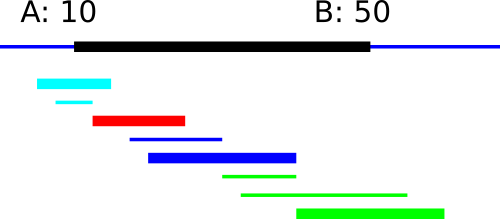
\includegraphics[width=.8\textwidth]{img/minimal_coverage_solution}\]
\end{frame}

\begin{frame}
  \frametitle{Greedy Search Example: Coin Change}

  Given a target value $V$ and a set of coin sizes $S$, select a group $C$ of coins (with repetition) that adds to $V$, so that the $|C|$ is minimum.
  \bigskip

  {\bf Example Input:} $V = 42, S = \{25, 10, 5, 1\}$\bigskip
    %{\small (a 1\$ coin means we can always make any value)}

  {\bf Example Output:} $25 + 10 + 5 + 1 + 1$: Size 5\bigskip

  \begin{block}{}
    What is the Greedy algorithm for this problem?
  \end{block}
\end{frame}

\begin{frame}{Greedy Search Example: Coin Change}{Wrong Answer!}
  \begin{block}{}
    A Greedy algorithm for Coin change would be to always take the largest coin, and reduce $V$ by the value of that coin:
    \begin{itemize}
      \item $V = 42, S = \{ 25, 10, 5, 1\}, C = \emptyset$, Take 25
      \item $V = 17, S = \{ 25, 10, 5, 1\}, C = \{25\}$, Take 10
      \item $V = 7, S = \{ 25, 10, 5, 1\}, C = \{25, 10\}$, Take 5
      \item $V = 2, S = \{ 25, 10, 5, 1\}, C = \{25, 10, 5\}$, Take 1
      \item $V = 1, S = \{ 25, 10, 5, 1\}, C = \{25, 10, 5, 1\}$, Take 1
    \end{itemize}
  \end{block}

  \begin{alertblock}{Wrong Answer!}
    \begin{itemize}
      \item $V = 6, S = \{4,3,1\}, C = \emptyset$, take 4
      \item $V = 2, S = \{4,3,1\}, C = \{4\}$, take 1
      \item $V = 1, S = \{4,3,1\}, C = \{4,1\}$, take 1
    \end{itemize}
  \end{alertblock}
\end{frame}

\begin{frame}
  \frametitle{Greedy Example 2 -- Load Balancing UVA 410}

  \begin{block}{Problem Description}

    \begin{itemize}
    \item There are $C$ chambers, and $S < 2C$ items.
    \item Each item has a positive weight $M_i$.
    \item You need to assign each item to a chamber in order to minimize ``imbalance''
    \end{itemize}

    \begin{equation*}
      A = \sum^S_{i=1}M_i/S
    \end{equation*}
    \begin{equation*}
      \text{Imbalance} = \sum^C_{i=1} |C_i - A|
    \end{equation*}
  \end{block}


  Can you figure out a greedy search solution?
\end{frame}


\begin{frame}
  \frametitle{Greedy Example 2 -- Load Balancing UVA 410}

  \begin{block}{Problem Description}
  You have C chambers, and S < 2C specimens with different positive
  weights. You need to decide where each specimen should go to
  minimize ``imbalance''.
  \end{block}

  Insights:

  \begin{itemize}
  \item A chamber with 1 individual is always better than a chamber
    with 0 individuals.

    \medskip

  \item Order of chambers does not matter.
  \end{itemize}
  %%% Make people think for a while here.
\end{frame}

\begin{frame}
  \frametitle{Greedy Example 2 -- Load Balancing UVA 410}

  \begin{block}{Problem Description}
  You have C chambers, and S < 2C specimens with different positive
  weights. You need to decide where each specimen should go to
  minimize ``imbalance''.
  \end{block}

  \vfill

  \structure{Greedy algorithm:} Order the individuals by weight, and
  put one in each chambers until the chambers are full, then add one
  in each chamber backwards.

  \bigskip

  A similar approach can be used to solve this week's problem ``Dragon
  of LooWater''.
\end{frame}

%%%%%%%%%%%%%%%%%%%%%%%%%%%%%%%%%%%%%%%%%%%%%%%%%%%%%%%%%%%%%%%%%%%%%%%%%%%%%%%%%%%%%%%%
%%% State Space Search
% UVA 11212 Editing a Book
% You can cut pages (in order) and paste them to correct the order of the book
% Report number of steps required.
% Upper bound: k-1 (paragraphs in the wrong position) - not correct answer, examples
% Calculations on the number of states for the problem (No solution given in the slides)
